\documentclass[12pt]{beamer}
\usetheme{Rec}
%\hypersetup{pdfpagemode=FullScreen}

\setbeamertemplate{footline}[text line]{} % makes the footer EMPTY
\useoutertheme[subsection=false]{smoothbars}

\usepackage{subfigure}
\usepackage{multicol}
\usepackage{graphicx}
\usepackage[all,knot]{xy}
\usepackage{url}
\usepackage{multimedia}
\usepackage{hyperref}
\usepackage{xcolor}
\usepackage{tabularx}

\usefonttheme{professionalfonts}
\usefonttheme{serif}
\usepackage{fontspec}
\setmainfont{Ubuntu}


\title{\Large git and Github}
\author{Tad Dallas}
\date{2018}




\begin{document}

\maketitle



\begin{frame}

	\begin{flushright}
	{\Large \textcolor{boss2}{Version control in 2 parts}}
	\end{flushright}

	\Huge	
	\textcolor{boss3}{git through command line} \\
	\bigskip
	\bigskip
	\textcolor{boss3}{git and Github} \\

\end{frame}






%%%%% git

\begin{frame}

	\begin{flushright}
	{\Large \textcolor{boss2}{What is git?}}
	\end{flushright}
  
\includegraphics[width=0.75\textwidth]{figs/Git-Logo-White.png}

\textcolor{boss3}{git was originally developed by Linus Torvalds to store and version Linux}


\end{frame}






\begin{frame}

	\begin{flushright}
		\Large \textcolor{boss2}{Who uses git?} 
	\end{flushright}
	
	\begin{center}
	  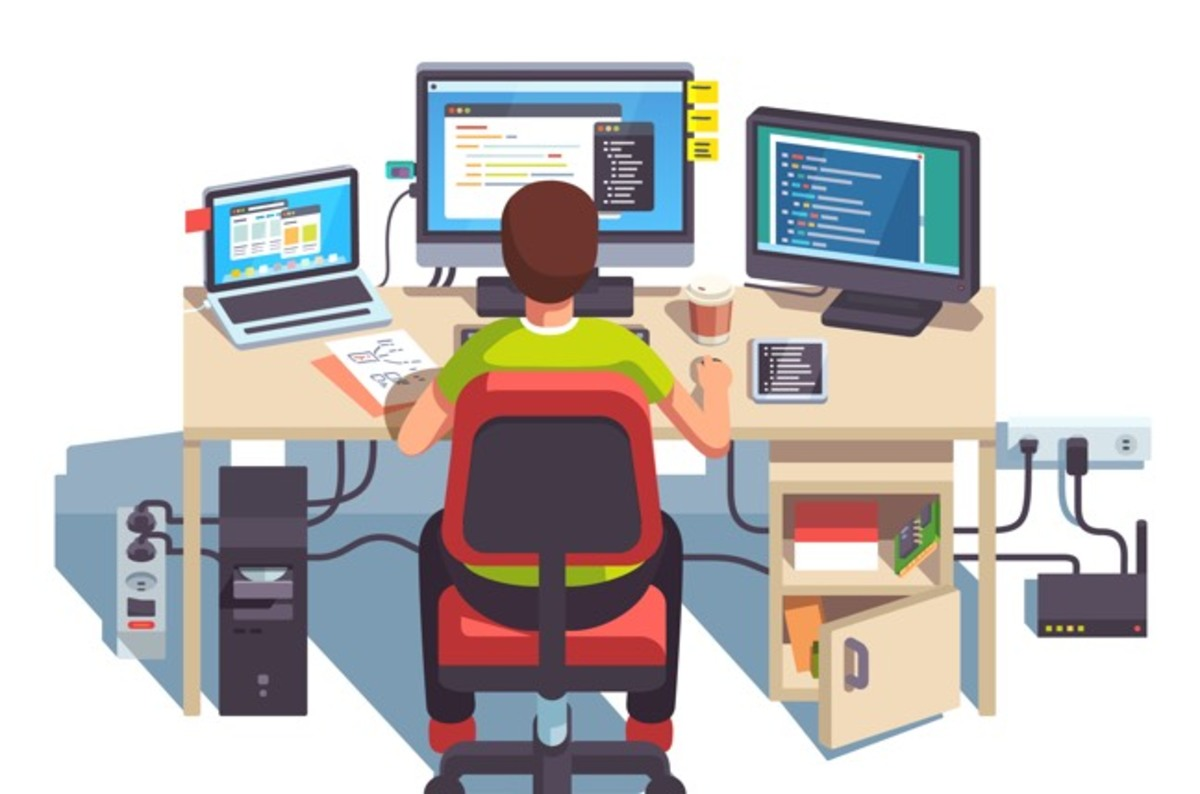
\includegraphics[width=0.75\textwidth]{figs/stereotype.jpg}
	\end{center}

\end{frame}




\begin{frame}

	\begin{flushright}
		\Large \textcolor{boss2}{Who uses git?} 
	\end{flushright}
	
	\begin{center}
	  
\includegraphics[width=0.75\textwidth]{figs/everyone.png}
	\end{center}

\end{frame}





\begin{frame}

	\Large \textcolor{boss3}{Version control:} \\

	\bigskip
	\bigskip

	\textcolor{boss4}{System that tracks changes to files, such that the user can recall different versions at any time}


\end{frame}






\begin{frame}

	\begin{flushright}
		\Large \textcolor{boss2}{Why use git?} 
	\end{flushright}

	\begin{center}
	  
\includegraphics[width=0.45\textwidth]{figs/phd101212s.pdf} \\
		https://phdcomics.com/
	\end{center}

\end{frame}






\begin{frame}

	\begin{flushright}
		\Large \textcolor{boss2}{How does git work?} 
	\end{flushright}

	\begin{center}
	  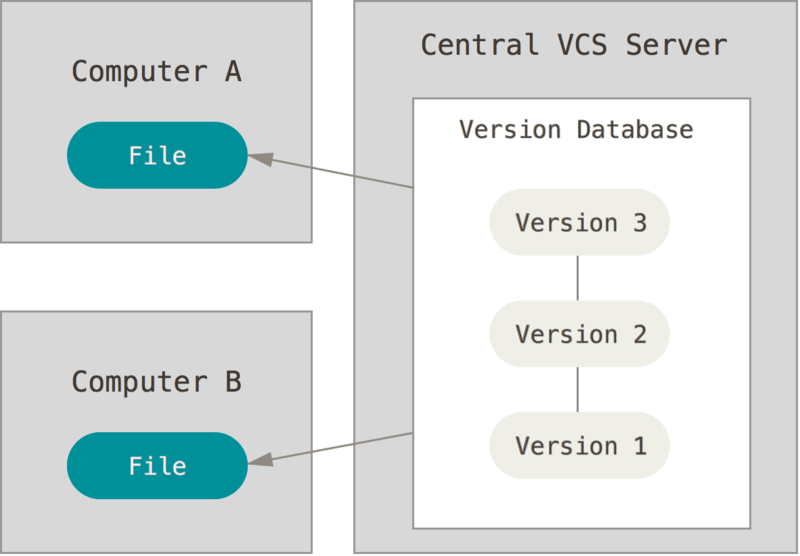
\includegraphics[width=0.75\textwidth]{figs/centralized.png}
		https://git-scm.com/
	\end{center}

\end{frame}











\begin{frame}

	\begin{flushright}
		\Large \textcolor{boss2}{How does git work?} 
	\end{flushright}

	\begin{center}
	  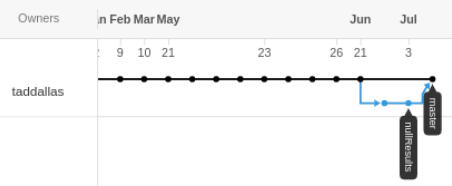
\includegraphics[width=\textwidth]{figs/gitHistory.png}
	\end{center}
% terms to touch on here: init, branch (master), commit, fork

\end{frame}





\begin{frame}

	\begin{flushright}
		\Large \textcolor{boss2}{How does git work?} 
	\end{flushright}

	\begin{center}
	  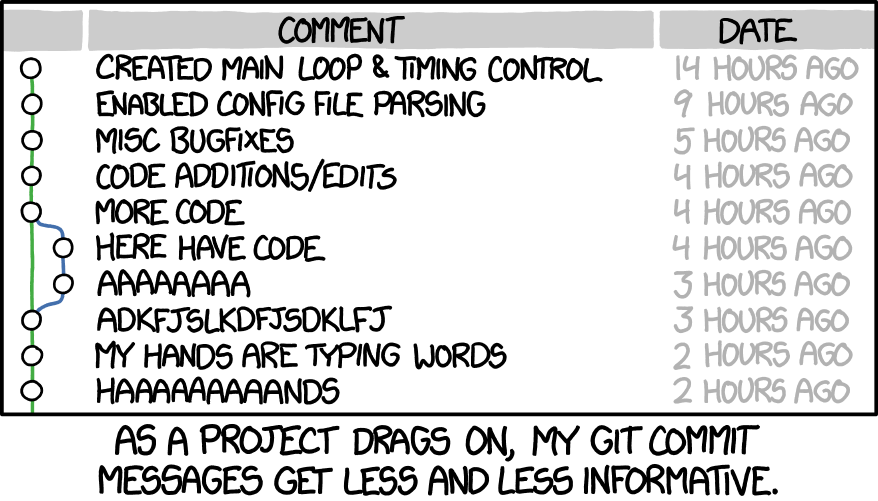
\includegraphics[width=\textwidth]{figs/commit.png}
		www.xkcd.com
	\end{center}

\end{frame}








\begin{frame}

	\begin{flushright}
		\Large \textcolor{boss2}{git} + \textcolor{boss4}{Rstudio} 
	\end{flushright}

	\begin{center}
	  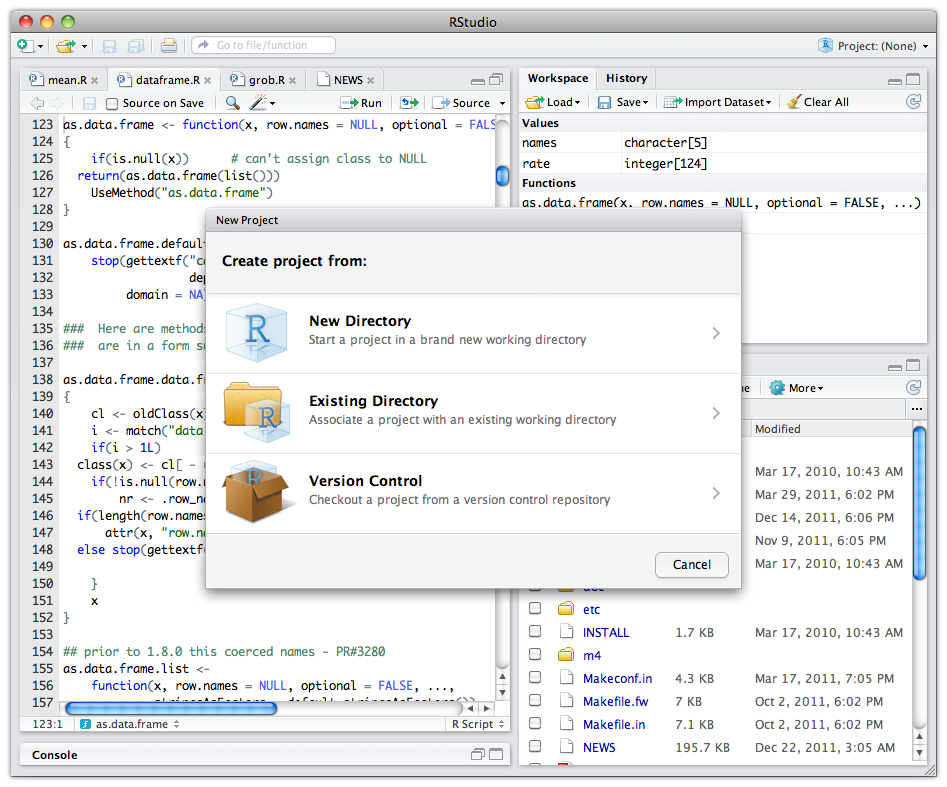
\includegraphics[width=0.9\textwidth]{figs/rstudio.png}
		https://jennybc.github.io/2014-05-12-ubc/r-setup.html
	\end{center}

\end{frame}








\begin{frame}

	\begin{flushright}
	\Large \textcolor{boss2}{A simple example} 
	\end{flushright}

	\textcolor{boss3}{Commands to cover:}

	\begin{itemize}
		\item init
		\item remote
		\item add
		\item commit
		\item status
		\item branch
		\item checkout
	\end{itemize}

\end{frame}





\begin{frame}

\end{frame}



































%%%%% Github


\begin{frame}

	\begin{flushright}
	\Large \textcolor{boss2}{What is Github?} 
	\end{flushright}

  \begin{center}
    
\includegraphics[width=\textwidth]{figs/github.png}
  \end{center}

	\textcolor{boss3}{git repository hosting service and development platform}

\end{frame}








\begin{frame}

	\begin{flushright}
  	\Large \textcolor{boss2}{Who uses Github?} 
	\end{flushright}

  \begin{center}
    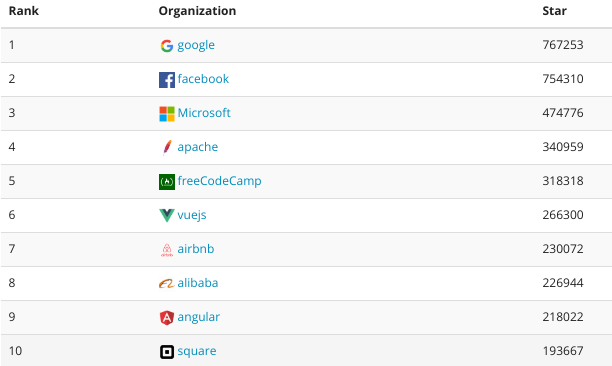
\includegraphics[width=\textwidth]{figs/topRepos.png}
  \end{center}

\end{frame}










\begin{frame}

	\begin{flushright}
  	\Large \textcolor{boss2}{Why use Github?} 
	\end{flushright}

	\begin{itemize}
		\item Open data/code facilitates contributions
		\item Initiate collaborations
		\item Track issues
		\item Assign tasks
		\item Track progress (milestones)
	\end{itemize}

	\bigskip
	\bigskip
	\textcolor{boss3}{Github repo != depositing data/code for manuscripts} \\

\end{frame}








\begin{frame}

	\begin{flushright}
  	\Large \textcolor{boss2}{A simple walkthrough} 
	\end{flushright}

	\begin{itemize}
		\item Set remote. 
		\item Push to repo. 
		\item File an issue.  
		\item Create a branch. 
		\item Create new content. 
		\item Push. 
		\item Pull request. 
		\item Look at commit history and diff. 
		\item Comment on a commit or issue. 
		\item Reference an issue or commit in a comment. 
		\item View milestones.  
	\end{itemize}

\end{frame}















\begin{frame}

	\begin{flushright}
		{\Large \textcolor{boss2}{git with Rstudio}} \\
	\end{flushright}
		jennybc.github.io/2014-05-12-ubc/ubc-r/session03\_git.html \\
		\bigskip
	\begin{flushright}
		{\Large \textcolor{boss2}{git tutorials}} \\
	\end{flushright}
		try.github.io/ \\
		guides.github.com/ \\
		www.codecademy.com/learn/learn-git \\
		\bigskip
	\begin{flushright}
		{\Large \textcolor{boss2}{git GUIs}} \\
	\end{flushright}
		git-scm.com/download/gui/windows	\\
		git-scm.com/download/gui/mac \\
		git-scm.com/download/gui/linux \\
\end{frame}















\begin{frame}

{\large \textcolor{recRed}{Contact}}

  \begin{flushright}
    \begin{tabular}{cl}
    \includegraphics[width=0.75cm]{figs/email.png} & \texttt{tad.dallas@helsinki.fi} \\
    \includegraphics[width=1.5cm]{figs/octocat.png} & \texttt{tad.dallas} \\
    \includegraphics[width=0.75cm]{figs/user.png} & \texttt{taddallas.github.io}\\
    \includegraphics[width=0.75cm]{figs/twitter.png} & \texttt{@taddallas} \\
   \end{tabular}
  \end{flushright}
\end{frame}

\end{document}
